\scanpage{166}
\uline{Sujets de recherches}

a) $\bigwedge^i$ dans catégories dérivées, $\lambda$-anneaux et structures annexes

\diagram{$\left\{\begin{array}{ll}
\text{b)}&\text{Dualité analytique}\\[1em]
\text{c)}&\text{Descente cohomologique et}\\
&\text{applications (finitude}\\
&\text{analytique et algébrique ....)}
\end{array}\right.$}

\diagram{$\left\{\begin{array}{ll}
\text{d)}&\text{Künneth pour complexes}\\
&\text{quasi-cohérents}\\[1em]
\text{e)}&\text{Dualité pour les complexes}\\
&\text{alg. différentiels, et}\\
&\text{site stratifiant ----}
\end{array}\right.$}

\figure{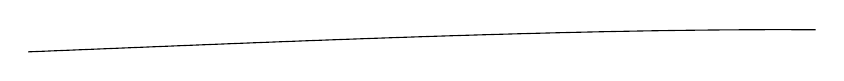
\begin{tikzpicture}\draw (0,0) .. controls (3,.12) and (7,.3) .. (10,.28);\end{tikzpicture}}

f) \deleted{Profondeurs cohomologiques et homotopiques, et ths de Lefschetz locaux et globaux.}

\figure{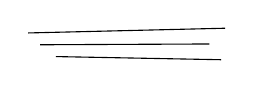
\begin{tikzpicture}\draw (0,.3)--(2.5,.36);\draw (.15,.15)--(2.3,.16);\draw (.35,0)--(2.45,-.04);\end{tikzpicture}}
\margin{165}
